
\documentclass[portrait,a4paper]{article}
\usepackage{tikz}
\usepackage{hyperref}
\usetikzlibrary{arrows,automata}
\usetikzlibrary{positioning}

\tikzstyle{master} x= [rectangle, rounded corners, minimum width=1cm, minimum height=1cm,text centered, text width=1.5cm, draw=black]


\tikzstyle{slave} x= [rectangle, rounded corners, minimum width=3cm, minimum height=1cm,text centered, text width=3cm, draw=black]

\tikzstyle{class} = [rectangle, rounded corners, minimum width=6cm, minimum height=1cm,text centered, text width=6 cm, draw=black]

\tikzstyle{interface} = [rectangle, rounded corners, minimum width=3cm, minimum height=1cm,text centered, draw=black]

\begin{document}
\Huge
\title{CLASS DIAGRAM}
\author{JOSE CARLOS MAYORAL BANOS}
\maketitle
\normalsize
\newpage
\begin{center}
\begin{tikzpicture}[node distance=2.5cm]
\node(superstart)[master] {robotsim};
\node(aa)[slave,below left of=superstart] {\hyperlink{page.3}{Actor}};
\node (a0) [slave,below right of=superstart] {\hyperlink{page.15}{Button}};
\node (a1) [slave,below of=aa] {\hyperlink{page.3}{LegoRobot}};
\node (a2) [slave,below of=a0] {\hyperlink{page.19}{LightAdapter}};
\node (a3) [slave,below of=a1] {\hyperlink{page.20}{main}};
\node (a4) [slave,below of=a2] {\hyperlink{page.21}{MotorPort}};
\node (a5) [slave,below of=a3] {\hyperlink{page.22}{PackageInfo}};
\node (a6) [slave,below of=a4] {\hyperlink{page.23}{RobotContext}};
\node (a7) [slave,below of=a5] {\hyperlink{page.25}{SensorPort}};
\node (a8) [slave,below of=a6] {\hyperlink{page.26}{SoundAdapter}};
\node (a9) [slave,below of=a7] {\hyperlink{page.28}{Tools}};
\node (a10) [slave,below of=a8] {\hyperlink{page.29}{TouchAdapter}};
\node (a11) [slave,below of=a9] {\hyperlink{page.31}{UltrasonicAdapter}};
\node (a12) [slave,below of=a10] {\hyperlink{page.31}{BrickButton}};
\node (a13) [slave,below of=a11] {\hyperlink{page.24}{}};
\draw (superstart) |- node{} (aa);
\draw (superstart) |- (a0);
\draw (superstart) |- (a1);
\draw (superstart) |- (a2);
\draw (superstart) |- (a3);
\draw (superstart) |- (a4);
\draw (superstart) |- (a5);
\draw (superstart) |- (a6);
\draw (superstart) |- (a7);
\draw (superstart) |- (a8);
\draw (superstart) |- (a9);
\draw (superstart) |- (a10);
\draw (superstart) |- (a11);
\end{tikzpicture}
\newpage
\begin{tikzpicture}[node distance=2.5cm]
\node(superstart1)[master,x=0] {Actor};
\node(bb)[slave,below left of=superstart1] {\hyperlink{page.4}{Part}};
\node (b0) [slave,below right of=superstart1] {\hyperlink{page.13}{Target}};
\node (b1) [slave,below of=bb] {\hyperlink{page.14}{Obstacle}};
\draw (superstart1) |- (b0);
\draw (superstart1) |- (b1);
\draw (superstart1) |- (bb);
\node(superstart2)[master,right of=superstart1,node distance=7cm] {\hyperlink{page.16}{LegoRobot}};
\node(bb)[slave,below left of=superstart2] {\hyperlink{page.17}{NxtRobot}};
\node (b0) [slave,below right of=superstart2] {\hyperlink{page.18}{TurtleRobot}};
\draw (superstart2) |- (bb);
\draw (superstart2) |- (b0);


\node(superstart3)[slave,below of=superstart1,node distance=10cm] {RobotContext};
\node(cc)[slave,below of=superstart3] {\hyperlink{page.24}{NxtContext}};
\draw (superstart3) -- (cc);



\end{tikzpicture}
\newpage

\begin{tikzpicture}[node distance=3 cm]

\node (init1) [slave,node distance=2] {Part};
\node (a1) [slave,below left of=init1] {\hyperlink{page.5}{ColorSensor}};
\node (a2) [slave,below right of=init1] {\hyperlink{page.6}{Gear}};
\node (a3) [slave,below of=a1] {\hyperlink{page.7}{LightSensor}};
\node (a4) [slave,below of=a2] {\hyperlink{page.8}{Motor}};
\node (a5) [slave,below of=a3] {\hyperlink{page.9}{NxtSoundSensor}};
\node (a6) [slave,below of=a4] {\hyperlink{page.10}{SoundSensor}};
\node (a7) [slave,below of=a5] {\hyperlink{page.11}{TouchSensor}};
\node (a8) [slave,below of=a6] {\hyperlink{page.12}{UltrasonicSensor}};
\draw (init1) |- (a1);
\draw (init1) |- (a2);
\draw (init1) |- (a3);
\draw (init1) |- (a4);
\draw (init1) |- (a5);
\draw (init1) |- (a6);
\draw (init1) |- (a7);
\draw (init1) |- (a8);

\end{tikzpicture}
\newpage

\begin{tikzpicture}[node distance=5 cm]
\node (in2) [class] {
\begin{tabular}{l}
  \textbf{class ColorSensor}\\\hline 
  \parbox{5.5cm}{\begin{itemize}
   \item \textbf{Fields}
   \item static int[][] colorCubes
   \item \textbf{Methods}
   \item public ColorSensor(SensorPort port)
   \item public ColorSensor()
   \item public int getLightValue()
   \item public java.awt.Color getColor()
   \item public int getColorID()
   \item public ColorLabel getColorLabel()
   \item public java.lang.String getColorStr()
   \item public static boolean inColorCube(java.awt.Color color,
                  int[] colorCube)
   \item public SensorPort getPort()
  \end{itemize}
  }
 \end{tabular}

 };
 \end{tikzpicture}
 \newpage
 \begin{tikzpicture}[node distance=3 cm]
\node (in3) [class,right of=init1] {
\begin{tabular}{l}
  \textbf{class Gear}\\\hline
\parbox{5.5cm}{\begin{itemize}
   \item \textbf{Methods}
   \item public Gear()
   \item public void forward()
   \item public void forward(int duration)
   \item public void backward()
   \item public void backward(int duration)
   \item public void stop()
   \item public void left()
   \item public void left(int duration)
   \item public void right()
   \item public void right(int duration)
   \item public void leftArc(double radius)
   \item public void leftArc(double radius,int duration)
   \item public void rightArc(double radius)
   \item public void rightArc(double radius,int duration)
   \item public void setSpeed(int speed)
   \item public int getSpeed()
   \item public boolean isMoving()
   \item public int getX()
   \item public int getY()
   \item public Location getLocation()
   \end{itemize}
  }
 \end{tabular}};
\end{tikzpicture}

\newpage

\begin{tikzpicture}[node distance=10 cm]

\node (in3) [class] {
\begin{tabular}{l}
  \textbf{class LightSensor}\\\hline 
  \parbox{5.5cm}{\begin{itemize}
   \item \textbf{Methods}
   \item public LightSensor(SensorPort port)
   \item public LightSensor()
   \item public void addLightListener(LightListener listener, int triggerLevel)
   \item public void addLightListener(LigthListener lister)
   \item public int setTriggerLevel(int triggerLevel)
   \item public int GetValue()
   \item public void activate (boolean enable)
   \item public SensorPort getPort()
  \end{itemize}
  }
 \end{tabular}
 };
\end{tikzpicture}

\newpage

\begin{tikzpicture}[node distance=10 cm]

 \node (in4) [class,right of=in3] {
\begin{tabular}{l}
  \textbf{class Motor}\\\hline 
  \parbox{5.5cm}{\begin{itemize}
   \item \textbf{Methods}
   \item public Motor()
   \item public void forward()
   \item public void backward()
   \item public void stop()
   \item public void setSpeed(int speed)
   \item public int getSpeed()
   \item public MotorPort getPort()
   \item boolean isMoving()
  \end{itemize}
  }
 \end{tabular}
 };
\end{tikzpicture}

\newpage

\begin{tikzpicture}

 \node (in5) [class] {
\begin{tabular}{l}
  \textbf{class NxtSoundSensor}\\\hline 
  \parbox{5.5cm}{\begin{itemize}
   \item \textbf{Methods}
   \item public NxtSoundSensor(SensorPort port)
   \item public void addSoundListener(SoundListener listener, int triggerLevel)
   \item public void addSoundListener(SoundListener listener)
   \item public int setTriggerLevel(int triggerLevel)
   \item public void sampleReceived(int count)
   \item public int getValue()
  \end{itemize}
  }
 \end{tabular}
};
\end{tikzpicture}

\newpage

\begin{tikzpicture}[node distance=10 cm]

 \node (in6) [class,right of=in5,node distance=7.5cm] {
\begin{tabular}{l}
  \textbf{class SoundSensor}\\\hline 
  \parbox{5.5cm}{\begin{itemize}
   \item \textbf{Methods}
   \item public SoundSensor(SensorPort port)
   \item public void addSoundListener(SoundListener listener, int triggerLevel)
   \item public void addSoundListener(SoundListener listener)
   \item public int setTriggerLevel(int triggerLevel)
   \item public void sampleReceived(int count)
   \item public int getValue()
  \end{itemize}
  }
 \end{tabular}};
\end{tikzpicture}

\newpage

\begin{tikzpicture}[node distance=10 cm]
 
 \node (in7) [class] {
\begin{tabular}{l}
  \textbf{class TouchSensor}\\\hline 
  \parbox{5.5cm}{\begin{itemize}
   \item \textbf{Methods}
   \item public TouchSensor(SensorPort port)
   \item public void addTouchListener(SoundListener listener)
   \item public void act()
   \item public boolean isPressed()
  \end{itemize}
  }
 \end{tabular}};
\end{tikzpicture}

\newpage

\begin{tikzpicture}[node distance=10 cm]
 \node (in8) [class] {
\begin{tabular}{l}
  \textbf{class UltrasonicSensor}\\\hline 
  \parbox{5.5cm}{\begin{itemize}
   \item \textbf{Methods}
   \item public UltrasonicSensor(SensorPort port)
   \item public void addUltrasonicListener(SoundListener listener,int triggerLevel)
   \item public void addUltrasonicListener(SoundListener listener)
   \item int setTriggerLevel(int triggerLevel)
   \item public int getDistance()
   \item public SensorPort getPort()
   \item public void setMeshTriangleColor(java.awt.Color color)
   \item public void setBeamAreaColor(java.awt.Color color)
   \item public void eraseBeamArea()
   \item public void setProximityCircleColor(java.awt.Color color)
   
  \end{itemize}
  }
 \end{tabular}};
\end{tikzpicture}

\newpage

\begin{tikzpicture}[node distance=10 cm]


 \node (in9) [class] {
\begin{tabular}{l}
  \textbf{class Target}\\\hline 
  \parbox{5.5cm}{\begin{itemize}
   \item \textbf{Methods}
   \item public Target(java.lang.String imageName,java.awt.Point[] mesh)
   \item public Target(java.awt.image.BufferredImage bi,java.awt.Point[] mesh) 
  \end{itemize}
  }
 \end{tabular}};
\end{tikzpicture}

\newpage

\begin{tikzpicture}[node distance=10 cm]


 \node (in10) [class] {
\begin{tabular}{l}
  \textbf{class Obstacle}\\\hline 
  \parbox{5.5cm}{\begin{itemize}
   \item \textbf{Methods}
   \item public Obstacle(java.lang.String imageName)
   \item public Obstacle(java.awt.image.BufferredImage bi)
  \end{itemize}
  }
 \end{tabular}};
\end{tikzpicture}

\newpage

\begin{tikzpicture}[node distance=10 cm]

 \node (in10) [class] {
\begin{tabular}{l}
  \textbf{class Button}\\\hline 
  \parbox{5.5cm}{\begin{itemize}
   \item \textbf{Fields}
   \item public static Button ESCAPE
   \item \textbf{Methods}
   \item public Button()
   \item public boolean isPressed()
   \item public boolean isDown()
  \end{itemize}
  }
 \end{tabular}};
\end{tikzpicture}

\newpage

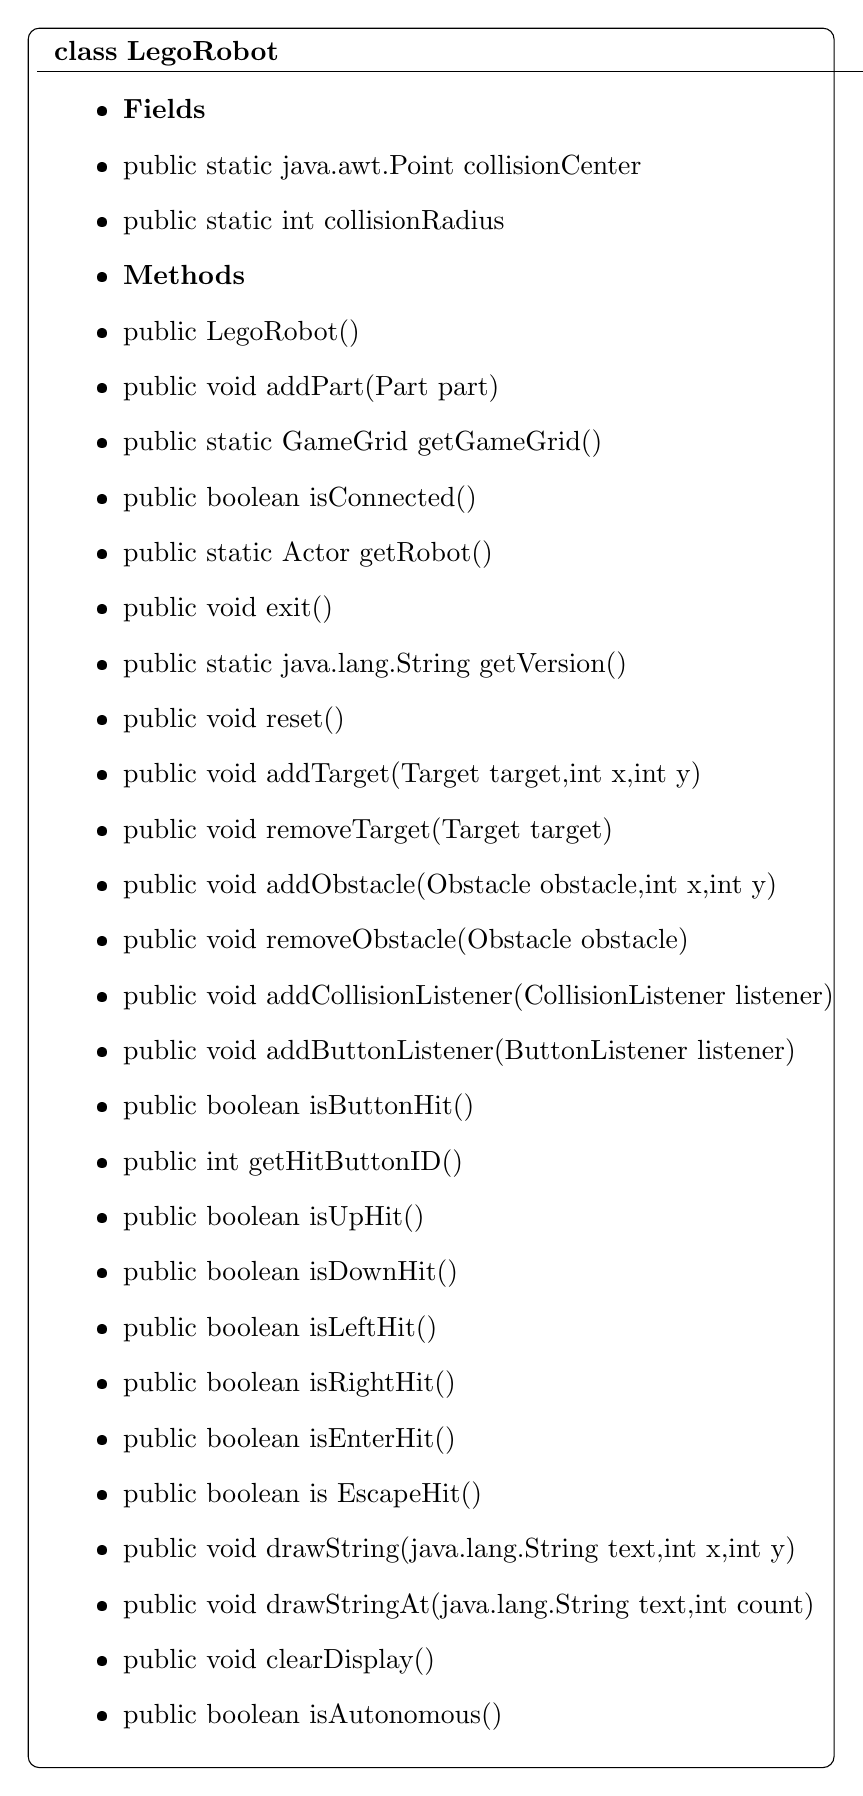
\begin{tikzpicture}[node distance=10 cm]


 \node (in11) [rectangle, rounded corners, minimum width=10cm, minimum height=1cm,text centered, text width=10 cm, draw=black] {
\begin{tabular}{l}
  \textbf{class LegoRobot}\\\hline 
  \parbox{10.5cm}{\begin{itemize}
   \item \textbf{Fields}
   \item public static java.awt.Point collisionCenter
   \item public static int collisionRadius
   \item \textbf{Methods}
   \item public LegoRobot()
   \item public void addPart(Part part)
   \item public static GameGrid getGameGrid()
   \item public boolean isConnected()
   \item public static Actor getRobot()
   \item public void exit()
   \item public static java.lang.String getVersion()
   \item public void reset()
   \item public void addTarget(Target target,int x,int y)
   \item public void removeTarget(Target target)
   \item public void addObstacle(Obstacle obstacle,int x,int y)
   \item public void removeObstacle(Obstacle obstacle)
   \item public void addCollisionListener(CollisionListener listener)
   \item public void addButtonListener(ButtonListener listener)
   \item public boolean isButtonHit()
   \item public int getHitButtonID()
   \item public boolean isUpHit()
   \item public boolean isDownHit()
   \item public boolean isLeftHit()
   \item public boolean isRightHit()
   \item public boolean isEnterHit()
   \item public boolean is EscapeHit()
   \item public void drawString(java.lang.String text,int x,int y)
   \item public void drawStringAt(java.lang.String text,int count)
   \item public void clearDisplay()
   \item public boolean isAutonomous()
  \end{itemize}
  }
 \end{tabular}};
\end{tikzpicture}

\newpage

\begin{tikzpicture}[node distance=10 cm]
 
 
 \node (in12) [class] {
\begin{tabular}{l}
  \textbf{class NxtRobot}\\\hline 
  \parbox{5.5cm}{\begin{itemize}
   \item \textbf{Methods}
   \item public NxtRobot()
  \end{itemize}
  }
 \end{tabular}};
\end{tikzpicture}

\newpage

\begin{tikzpicture}[node distance=10 cm]
 
 \node (in13) [class] {
\begin{tabular}{l}
  \textbf{class TurtleRobot}\\\hline 
  \parbox{5.5cm}{\begin{itemize}
   \item \textbf{Methods}
   \item public TurtleRobot()
   \item public void setTurtleSpeed(int speed)
   \item public int getTurtleSpeed()
   \item public void forward()
   \item public void forward(int steps)
   \item public void backward()
   \item public void backward(int steps)
   \item public void right(double angles)
   \item public void right()
   \item public void left(double angle)
   \item public void left()
   \item public Gear getGear()
  \end{itemize}
  }
 \end{tabular}};
\end{tikzpicture}

\newpage

\begin{tikzpicture}[node distance=10 cm]
 
  \node (in14) [class] {
\begin{tabular}{l}
  \textbf{class LightAdapter}\\\hline 
  \parbox{5.5cm}{\begin{itemize}
   \item \textbf{Methods}
   \item public LightAdapter()
   \item public void bright(SensorPort port,int level)
   \item public void dark(SensorPort port,int level)
  \end{itemize}
  }
 \end{tabular}};
\end{tikzpicture}

\newpage

\begin{tikzpicture}[node distance=10 cm]
 
  \node (in15) [class] {
\begin{tabular}{l}
  \textbf{class main}\\\hline 
  \parbox{5.5cm}{\begin{itemize}
   \item \textbf{Methods}
   \item public static void main(java.lang.String[] args)
  \end{itemize}
  }
 \end{tabular}};
\end{tikzpicture}

\newpage

\begin{tikzpicture}[node distance=10 cm]
 
  \node (in16) [class] {
\begin{tabular}{l}
  \textbf{class MotorPort}\\\hline 
  \parbox{5.5cm}{\begin{itemize}
   \item \textbf{Fields}
   \item public static Motor A
   \item public static Motor B
   \item public static Motor C
   \end{itemize}
  }
 \end{tabular}};
\end{tikzpicture}

\newpage

\begin{tikzpicture}[node distance=10 cm]
 
  \node (in17) [class] {
\begin{tabular}{l}
  \textbf{class PackageInfo}\\\hline 
  \parbox{5.5cm}{\begin{itemize}
   \item \textbf{Fields}
   \item public static java.lang.String VERSION
   \item \textbf{Methods}
   \item public PackageInfo()
  \end{itemize}
  }
 \end{tabular}};
\end{tikzpicture}

\newpage

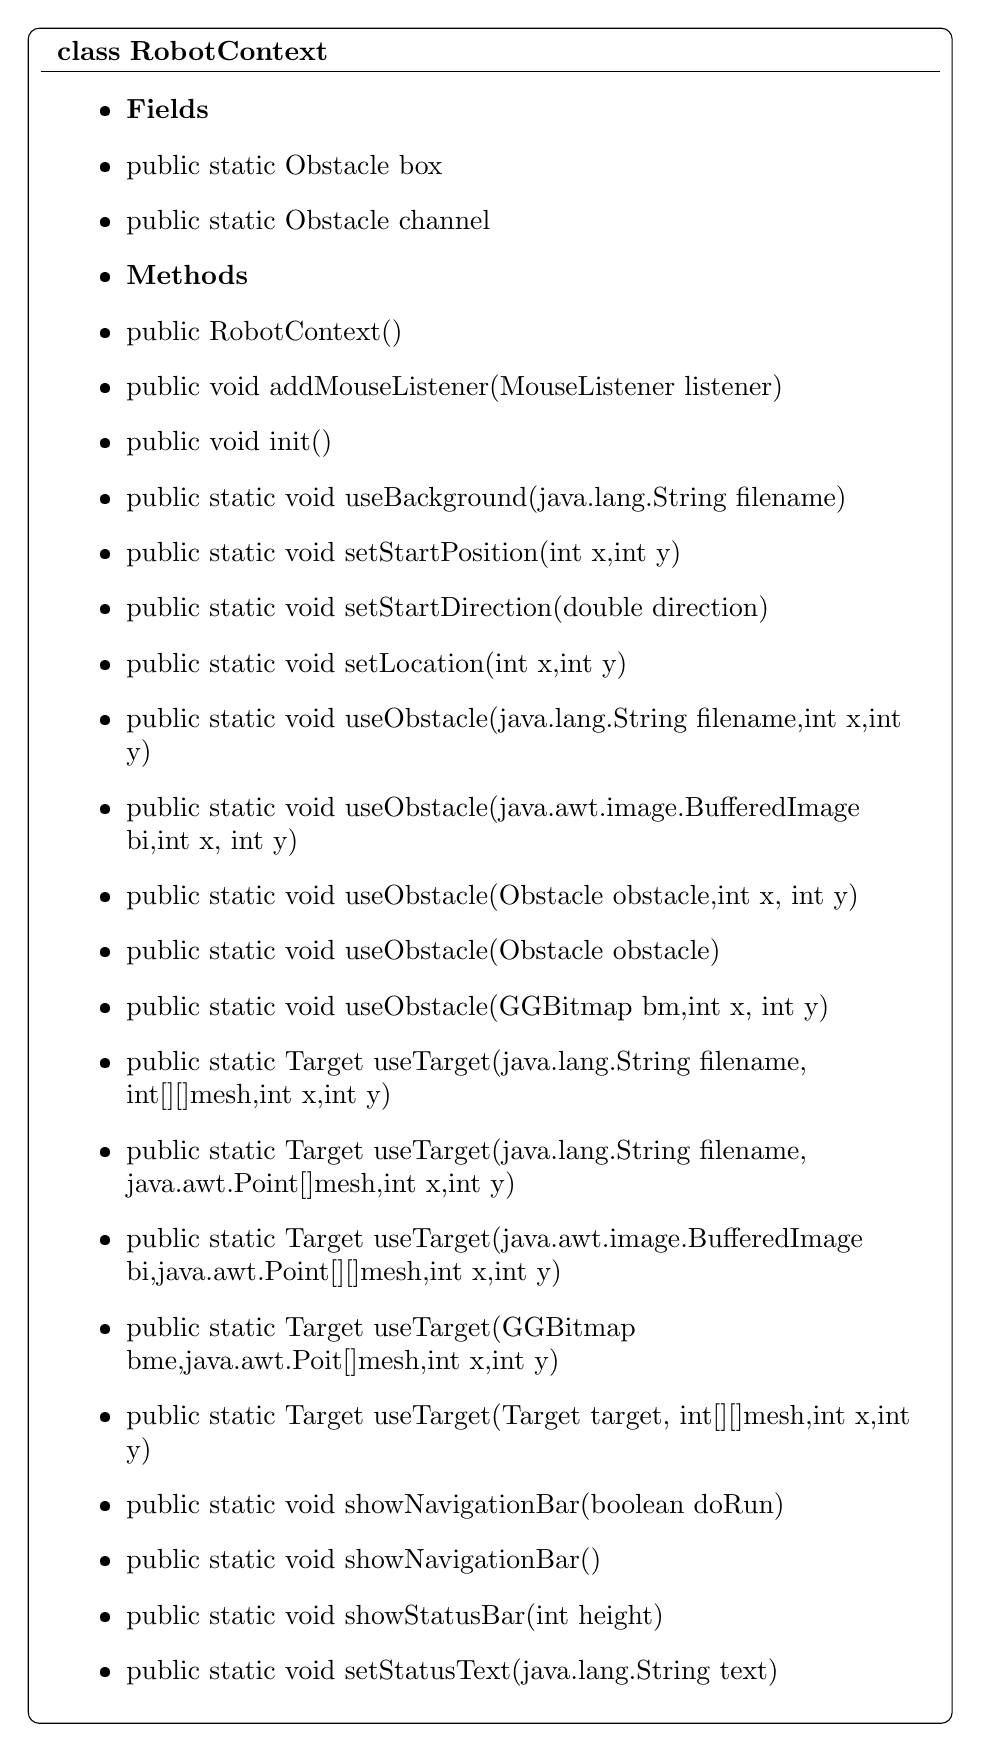
\begin{tikzpicture}[node distance=10 cm]
 
  \node (in18) [rectangle, rounded corners, minimum width=11.5cm, minimum height=1cm,text centered, text width=11.5 cm, draw=black] {
\begin{tabular}{l}
  \textbf{class RobotContext}\\\hline 
  \parbox{11cm}{\begin{itemize}
   \item \textbf{Fields}
   \item public static Obstacle box
   \item public static Obstacle channel
   \item \textbf{Methods}
   \item public RobotContext()
   \item public void addMouseListener(MouseListener listener)
   \item public void init()
   \item public static void useBackground(java.lang.String filename)
   \item public static void setStartPosition(int x,int y)
   \item public static void setStartDirection(double direction)
   \item public static void setLocation(int x,int y)
   \item public static void useObstacle(java.lang.String filename,int x,int y)
   \item public static void useObstacle(java.awt.image.BufferedImage bi,int x, int y)
   \item public static void useObstacle(Obstacle obstacle,int x, int y)
   \item public static void useObstacle(Obstacle obstacle)
   \item public static void useObstacle(GGBitmap bm,int x, int y)
   \item public static Target useTarget(java.lang.String filename, int[][]mesh,int x,int y)
   \item public static Target useTarget(java.lang.String filename, java.awt.Point[]mesh,int x,int y)
   \item public static Target useTarget(java.awt.image.BufferedImage bi,java.awt.Point[][]mesh,int x,int y)
   \item public static Target useTarget(GGBitmap bme,java.awt.Poit[]mesh,int x,int y)
   \item public static Target useTarget(Target target, int[][]mesh,int x,int y)
   \item public static void showNavigationBar(boolean doRun)
   \item public static void showNavigationBar()
   \item public static void showStatusBar(int height)
   \item public static void setStatusText(java.lang.String text)  
   
  \end{itemize}
  }
 \end{tabular}};
\end{tikzpicture}
\newpage
\begin{tikzpicture}
  \node (in19) [class] {
\begin{tabular}{l}
  \textbf{class NxtContext}\\\hline 
  \parbox{5.5cm}{\begin{itemize}
   \item \textbf{Methods}
   \item public NxtContext()
  \end{itemize}
  }
 \end{tabular}};
\end{tikzpicture}

\newpage

\begin{tikzpicture}[node distance=10 cm]
 
   \node (in20) [class] {
\begin{tabular}{l}
  \textbf{class SensorPort}\\\hline 
  \parbox{5.5cm}{\begin{itemize}
   \item \textbf{Fields}
   \item static SensorPort S1
   \item static SensorPort S2
   \item static SensorPort S3   
   \item static SensorPort S4
  \end{itemize}
  }
 \end{tabular}};
\end{tikzpicture}

\newpage

\begin{tikzpicture}[node distance=10 cm]

\node (in21) [class] {
\begin{tabular}{l}
  \textbf{class SoundAdapter}\\\hline 
  \parbox{5.5cm}{\begin{itemize}
   \item \textbf{Methods}
   \item public SoundAdapter()
   \item public void loud(SensorPort port,int level)
      \item public void quiet(SensorPort port,int level)
   
  \end{itemize}
  }
 \end{tabular}};
\end{tikzpicture}

\newpage

\begin{tikzpicture}[node distance=10 cm]
 
\node (in22) [class] {
\begin{tabular}{l}
  \textbf{class SoundListener}\\\hline 
  \parbox{5.5cm}{\begin{itemize}
   \item \textbf{Methods}
   \item public void loud(SensorPort port,int level)
      \item public void quiet(SensorPort port,int level)
   
  \end{itemize}
  }
 \end{tabular}};
\end{tikzpicture}

\newpage

\begin{tikzpicture}[node distance=10 cm]
 
\node (in23) [class] {
\begin{tabular}{l}
  \textbf{class Tools}\\\hline 
  \parbox{5.5cm}{\begin{itemize}
   \item \textbf{Methods}
   \item public Tools()
   \item public static void startTimer()
      \item public static long getTime()
      \item public static void delay(int duration)
         
  \end{itemize}
  }
 \end{tabular}};
\end{tikzpicture}

\newpage

\begin{tikzpicture}[node distance=10 cm]
 

\node (in24) [class] {
\begin{tabular}{l}
  \textbf{class TouchAdapter}\\\hline 
  \parbox{5.5cm}{\begin{itemize}
   \item \textbf{Methods}
   \item public TouchAdapter()
   \item public void pressed(SensorPort port)
   \item public void released(SensorPort port)
         
  \end{itemize}
  }
 \end{tabular}};
\end{tikzpicture}

\newpage

\begin{tikzpicture}[node distance=10 cm]


\node (in25) [class] {
\begin{tabular}{l}
  \textbf{class TouchListener}\\\hline 
  \parbox{5.5cm}{\begin{itemize}
   \item \textbf{Methods}
   \item public void pressed(SensorPort port)
   \item public void released(SensorPort port)
         
  \end{itemize}
  }
 \end{tabular}};
\end{tikzpicture}

\newpage

\begin{tikzpicture}[node distance=10 cm]

\node (in26) [class] {
\begin{tabular}{l}
  \textbf{class UltrasonicAdapter}\\\hline 
  \parbox{5.5cm}{\begin{itemize}
   \item \textbf{Methods}
   \item public UltrasonicAdapter()
   \item public void far(SensorPort port,int value)
   \item public void near(SensorPort port,int value)
         
  \end{itemize}
  }
 \end{tabular}};
\end{tikzpicture}

\newpage

\begin{tikzpicture}[node distance=10 cm]

\node (in27) [class] {
\begin{tabular}{l}
  \textbf{class UltrasonicListener}\\\hline 
  \parbox{5.5cm}{\begin{itemize}
   \item \textbf{Methods}
   \item public void far(SensorPort port,int value)
   \item public void near(SensorPort port,int value)
         
  \end{itemize}
  }
 \end{tabular}};
\end{tikzpicture}

\newpage

\begin{tikzpicture}[node distance=10 cm]




\node (in28) [class] {
\begin{tabular}{l}
  \textbf{class BrickButton}\\\hline 
  \parbox{5.5cm}{\begin{itemize}

   \item \textbf{Fields}
   \item static final int IDDOWN
   \item static final int IDENTER
   \item static final int IDESCAPE
   \item static final int IDLEFT
   \item static final int IDRIGHT
   \item static final int IDUP      
         
  \end{itemize}
  }
 \end{tabular}};
\end{tikzpicture}

\newpage

\begin{tikzpicture}[node distance=10 cm]





\node (in29) [class] {
\begin{tabular}{l}
  \textbf{class ButtonListener}\\\hline 
  \parbox{5.5cm}{\begin{itemize}
   \item \textbf{Methods}
   \item public void ButtonHit(int buttonID)
         
  \end{itemize}
  }
 \end{tabular}};
\end{tikzpicture}

\newpage

\begin{tikzpicture}[node distance=10 cm]


\node (in30) [class] {
\begin{tabular}{l}
  \textbf{class CollissionListener}\\\hline 
  \parbox{5.5cm}{\begin{itemize}
   \item \textbf{Methods}
   \item public void collide()
         
  \end{itemize}
  }
 \end{tabular}};
\end{tikzpicture}

\newpage

\begin{tikzpicture}[node distance=10 cm]
 
 \node (in31) [class] {
\begin{tabular}{l}
  \textbf{class LightListener}\\\hline 
  \parbox{5.5cm}{\begin{itemize}
   \item \textbf{Methods}
   \item public void bright(SensorPort port,int level)
   \item public void dark(SensorPort port,int level)         
  \end{itemize}
  }
 \end{tabular}};

\end{tikzpicture}

\newpage

\begin{tikzpicture}[node distance=10 cm]

\node (in32) [class] {
\begin{tabular}{l}
  \textbf{class MouseListener}\\\hline 
  \parbox{5.5cm}{\begin{itemize}
   \item \textbf{Methods}
	\item void mousePressed(GameGrid gg,
                int x,
                int y)
   \item	 void mouseReleased(GameGrid gg,
                 int x,
                 int y)
   \item void mouseDragged(GameGrid gg,
                int x,
                int y)
  \end{itemize}
  }
 \end{tabular}};

\end{tikzpicture}

%\draw (superstart) -> (start);
%\draw (start) -> (in1);

\end{center}
\end{document}






